% Chapter 4

\chapter{Anisotropic Flow} % Main chapter title
\label{sect:flow}
%----------------------------------------------------------------------------------------
\begin{figure}[htbp!]
  \centering
    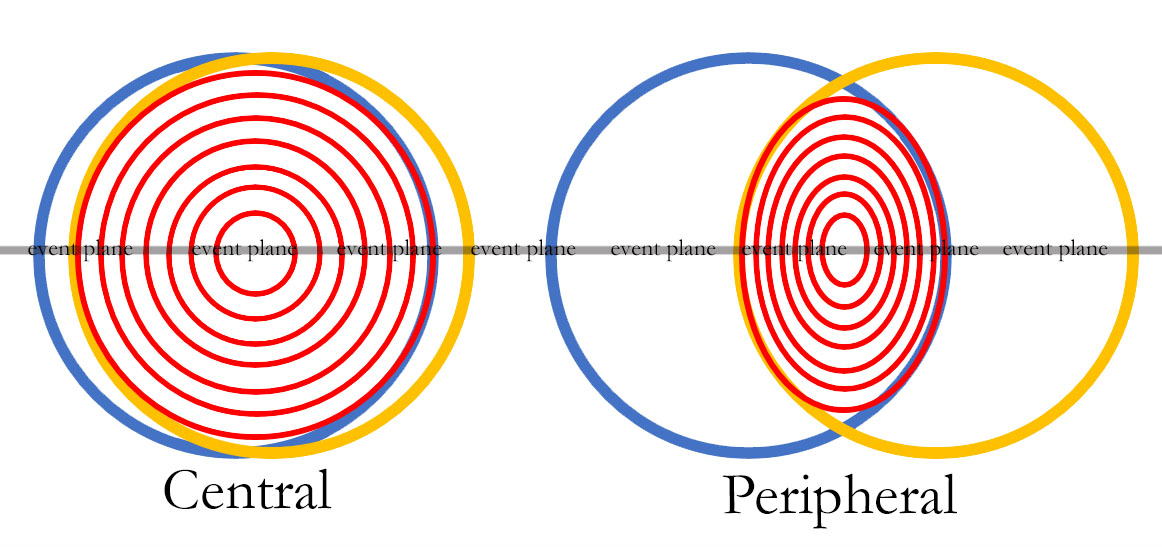
\includegraphics[width=0.6\textwidth]{Figures/pressuregradientsvscent.jpg}
    
        \rule{35em}{0.5pt}
  \caption[Pressure gradients in central versus peripheral collisions.]{Pressure gradients in central versus peripheral collisions. The ellipsoidal ion collision anisotropy corresponds to a pressure anisotropy in the QGP thus leading to an elliptic momentum anisotropy of particles produced in the azimuth.}
  \label{fig:pressuregradients}
\end{figure}


In the moments immediately after a collision event, the outwardly expanding behavior of the newly formed QGP can be studied to better understand the QCD processes that take place both during formation as well what happens as this QGP dissipates. The initial geometric shape of the created QGP is dependent on the collision's centrality (sect. \ref{sect:centrality}). Peripheral events cause a pressure anisotropy resulting in differential pressure gradients in the QGP. These pressures are strongest along the waist of the collision and weakest at the poles. Because of this, though it expands in all directions it is the expansion about the azimuth that best describes the behavior of this fluid. Often physicists like to describe the behavior of phenomena using a series expansion of orthogonal functions. Since the azimuthal angle runs from $0$ to $2 \pi$, this azimuthal expansion can be treated as a harmonic function which lends itself well to parameterization using a Fourier series. Recall that a Fourier series can be used to approximate the shape of a periodic function, $f(x)$, over a fixed period, $L$:

\begin{equation}
f(x) = \sum^{\infty}_{n=-\infty} A_{n} e^{i(2 \pi n x / L)}
\end{equation}
where
\begin{equation}
A_{n} = \frac{1}{L} \int^{L}_{0} f(\phi) e^{-i(2 \pi n x / L)} dx
\end{equation}

are said to be the Fourier \textbf{coefficients} or often, since they approximate harmonic functions, Fourier \textbf{harmonics}. For azimuthal periodicity, $L=2\pi$ and these equations become: 

\begin{equation}
f(\phi) = \sum^{\infty}_{n=-\infty} A_{n} e^{i(n \phi)}
\end{equation}
where
\begin{equation}
A_{n} = \frac{1}{2\pi} \int^{-\pi}_{\pi} f(\phi) e^{-i(n \phi)} d\phi
\end{equation}

These coefficients describe the amount a particular harmonic's functional shape contributes to the overall shape of the periodic function. We know that the exponential term can be written as the sum of a real cosine term and an imaginary sine term:

\begin{equation}
f(\phi) = \sum^{\infty}_{n=0} A_{n} cos ( n \phi) + i \sum^{\infty}_{n=0} B_{n} sin (n \phi)
\end{equation}
where
\begin{equation}
A_{n} = \frac{1}{2\pi} \int^{-\pi}_{\pi} f(\phi) cos (n \phi) d\phi
\end{equation}
and
\begin{equation}
B_{n} = \frac{1}{2\pi} \int^{-\pi}_{\pi} f(\phi) sin (n \phi) d\phi 
\end{equation}

\begin{figure}[htbp!]
  \centering
  \rule{35em}{0.5pt}
    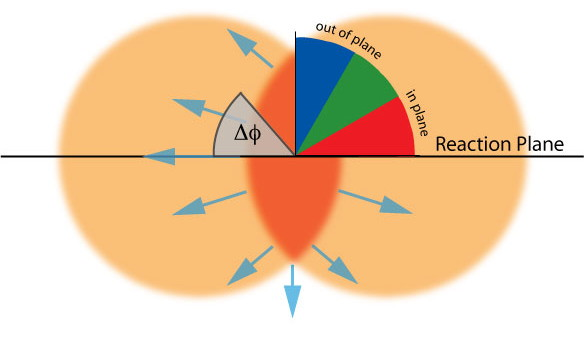
\includegraphics[width=0.7\textwidth]{Figures/RP_InOutPlane_3.jpg}
        
  \caption[Reaction plane coordinates.]{Reaction plane coordinates. $\phi = 0$ is oriented along the reaction plane therefore track vectors with $\Delta\phi$ values at $\pi/2$ and $3 \pi / 2$ correspond to particles produced out of the event plane and $\Delta\phi$ values of $0$ and $\pi$ correspond to vectors in the event plane.}
  \rule{35em}{0.5pt}
  \label{fig:dphiep}
\end{figure}


Since we define $\phi=0$ to be along the waist of the ellipsoidal shaped QGP and not at the poles (see fig \ref{fig:dphiep}), odd function contributions (sine terms, $B_{n}$) to the Fourier series can all be ignored. Therefore, if we wish to approximate the shape of the outgoing flow from the QGP, we can define the rate of change of outgoing particle tracks vs transverse momentum and approximate it with a Fourier series. Flow anisotropy of the QGP can then be written as:
\begin{equation}
E \frac{d^{3}N}{dp^{3}} = \frac{1}{2 \pi} \frac{d^{2}N}{p_{T} dp_{T}dy}\Big( 1 + \sum^{\infty}_{n=1} 2 v_{n} \cos\big(n \Delta \phi)\big) \Big),
\end{equation}
where:
\begin{equation}
v_{n} = \bigg \langle cos \Big( n \Delta\phi \Big) \bigg \rangle
\end{equation}
are the n-th order Fourier coefficients that describe the azimuthal shape of the QGP's outward expansion and $\Delta \phi = \phi_{lab} - \Psi_{RP}$ is the azimuthal angle with respect to the reaction plane angle relative measured in the lab coordinate system, changing the lab coordinate phi to the angle phi with respect to the event plane. Each n-th order coefficient scales the amount of expansion that behaves like $cos$ $nx$.

\begin{figure}[htbp!]
  \centering
    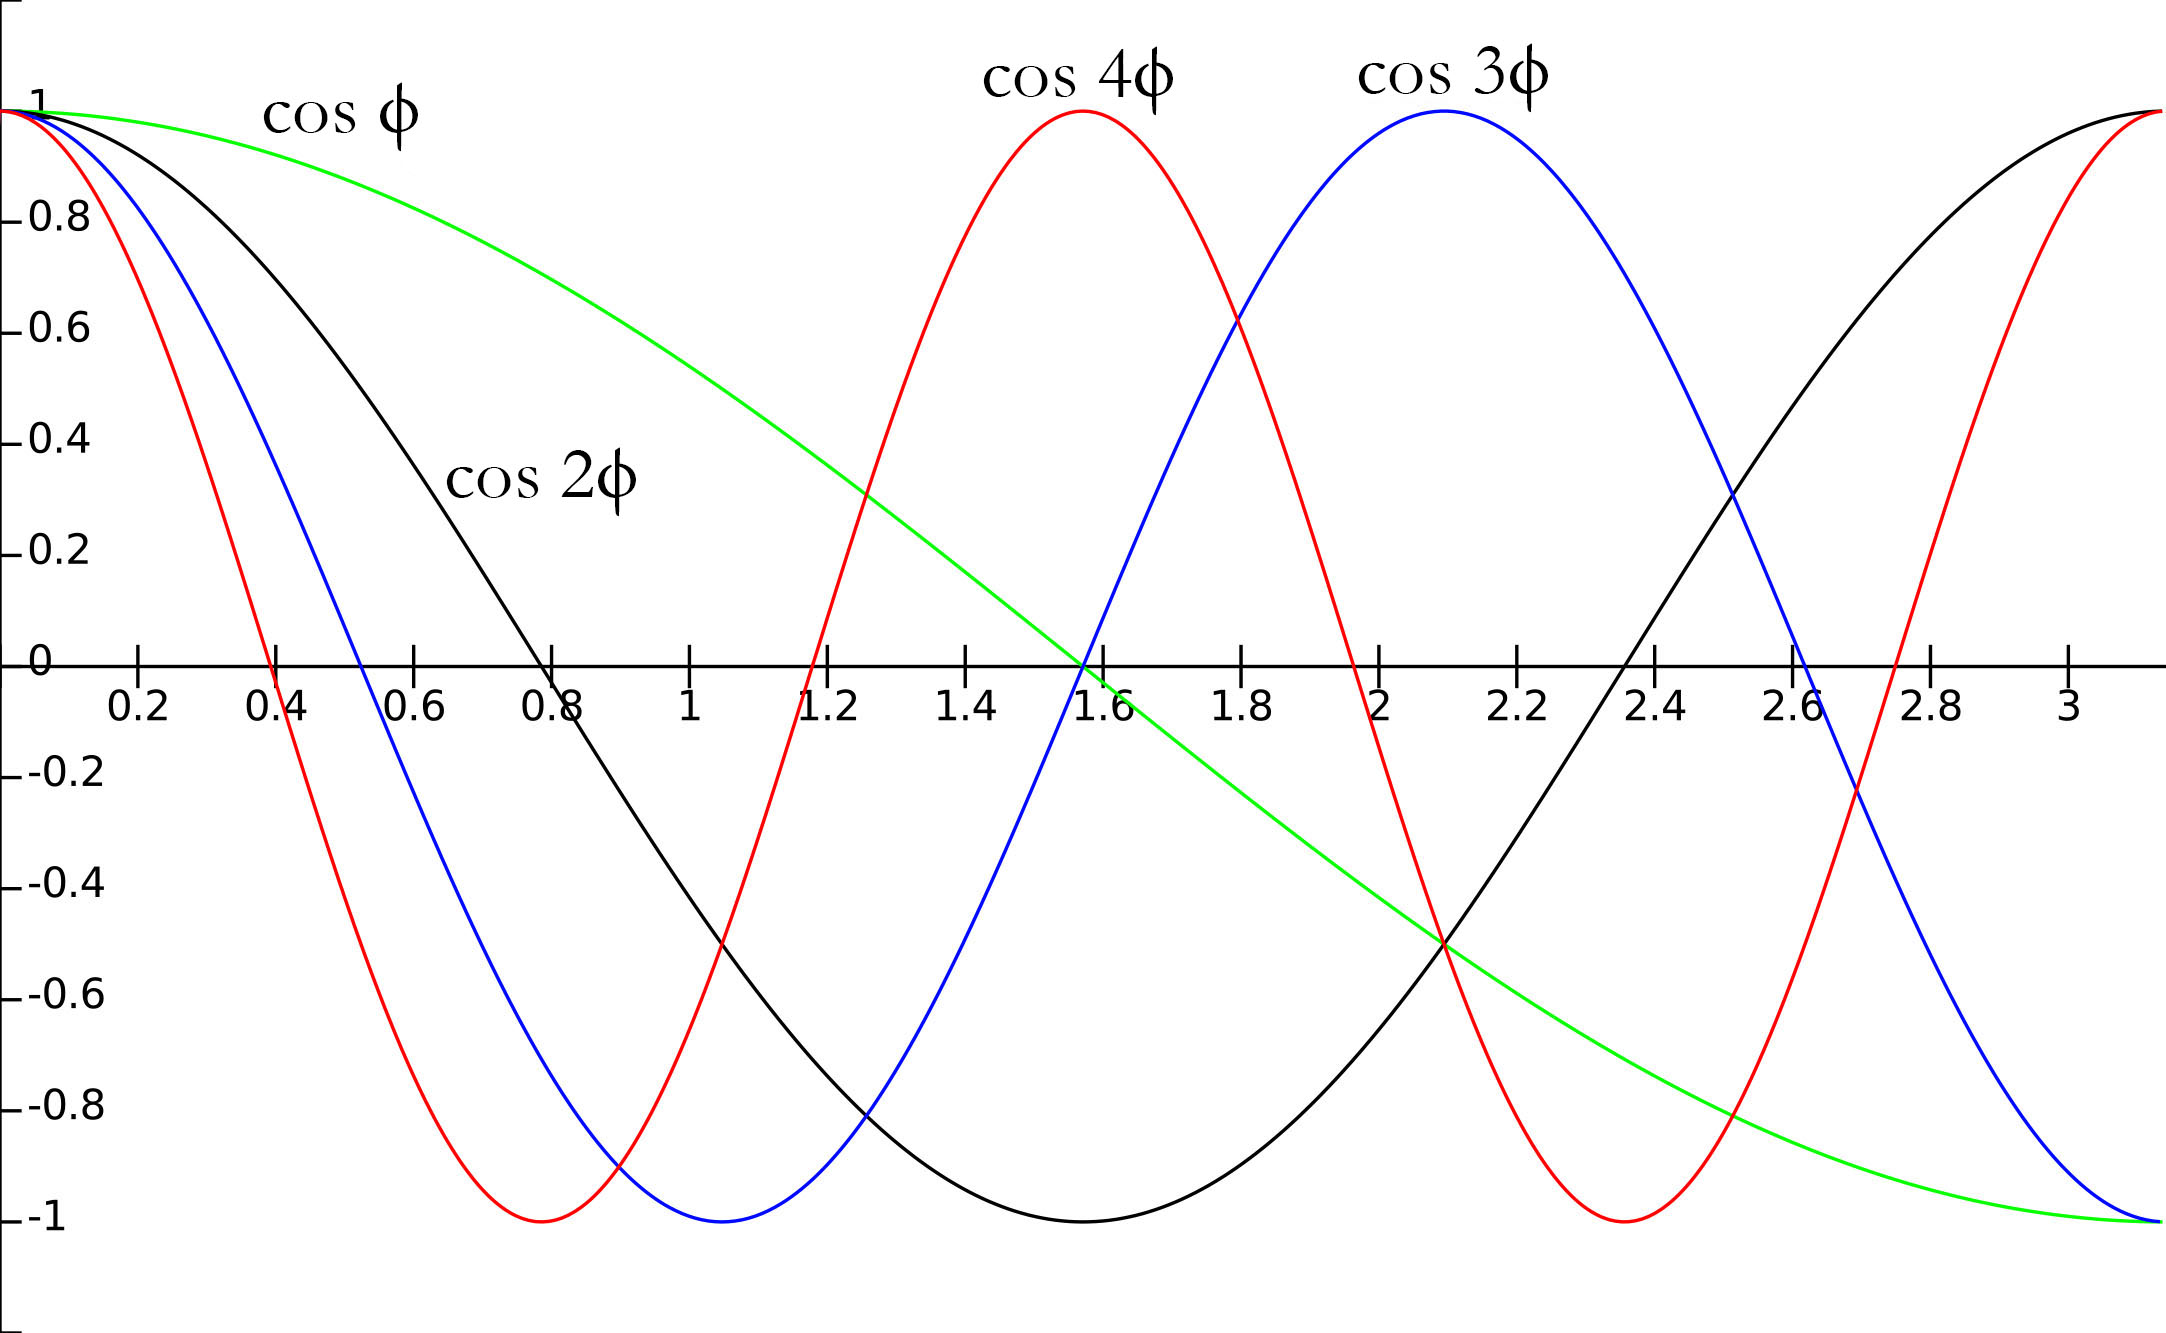
\includegraphics[width=0.8\textwidth]{Figures/fouriercosines.jpg}
    \rule{35em}{0.5pt}
  \caption[Plots of the first four harmonics of a cosine series]{Plots of the first four harmonics of a cosine series}
  \label{fig:fouriercosines}
\end{figure}

From studying the behavior of these various harmonics we can see that $n=0$ corresponds to a constant term since $\cos{0} = 1$ for $n=1$. Furthermore, $cos x$ is a maximum at $\phi=0$ and a minimum at $\phi = \pi$ which would correspond to a collective flow in the $\phi=0$ direction. Therefore the $n=1$ flow coefficient is often called \textit{directed flow}. For the case of $n=2$ we see that again there is a maximum at $\phi=0$ and another at $\phi=\pi$ which corresponds to maximal flow along the event plane of the ellipsoidal QGP. This anisotropic expansion that is strongest along the reaction plane in an elliptical collective flow, a term which is shortened to \textit{elliptic flow}. There are higher order harmonics which can describe various other phenomena of QGP flow which are beyond the scope of this analysis.



\pagebreak
\pagebreak
